\section{CarryBotsの開発}
本章では,製作したロボットの概要について述べる.

\subsection{ロボットの概要}
前章で述べた式から,上下のロボット間の摩擦を上げることに着目する.
また,他のロボットに乗り上げることを実現する機構として,
\reffig{rack-pinion}に示すラックレール・ピニオン車輪構造を用いた.
さらに,ピニオン車輪の歯先に滑りにくい,軟質樹脂製パッドをつけ,車輪のグリップを高める.
そして,ロボットが物体の姿勢を検知するためのセンサとして,\reffig{limit-switch}に示すようにリミットスイッチを採用した.
このラックレール,ピニオン車輪と物体の姿勢を検知するセンサを用いて製作したロボットを\reffig{carrybot}に示す.
使用するモータは一つのみで,ギアを通じて車軸へ動力を伝達する.

\begin{figure}[tb]
  \begin{minipage}[b]{0.6\columnwidth}
  \centering
  \includegraphics[width=0.95\columnwidth]{figures/rack-pinion.pdf}
  \subcaption{Rack-rail \& pinion-wheel}
  \label{fig:rack-pinion}
 \end{minipage}%
 \begin{minipage}[b]{0.4\columnwidth}
  \centering
  \includegraphics[width=0.95\columnwidth]{figures/limit-switch.pdf}
  \subcaption{Posture detector}
  \label{fig:limit-switch}
 \end{minipage}
 \caption{Proposed mechanism}
 \label{fig:mechanism}
\end{figure}
\begin{figure}[tb]
  \begin{minipage}[b]{0.5\columnwidth}
  \centering
  \includegraphics[width=0.9\columnwidth]{figures/carrybot-diagonal.pdf}
  \subcaption{Diagonal view}
  \label{fig:diagonal}
 \end{minipage}%
 \begin{minipage}[b]{0.5\columnwidth}
  \centering
  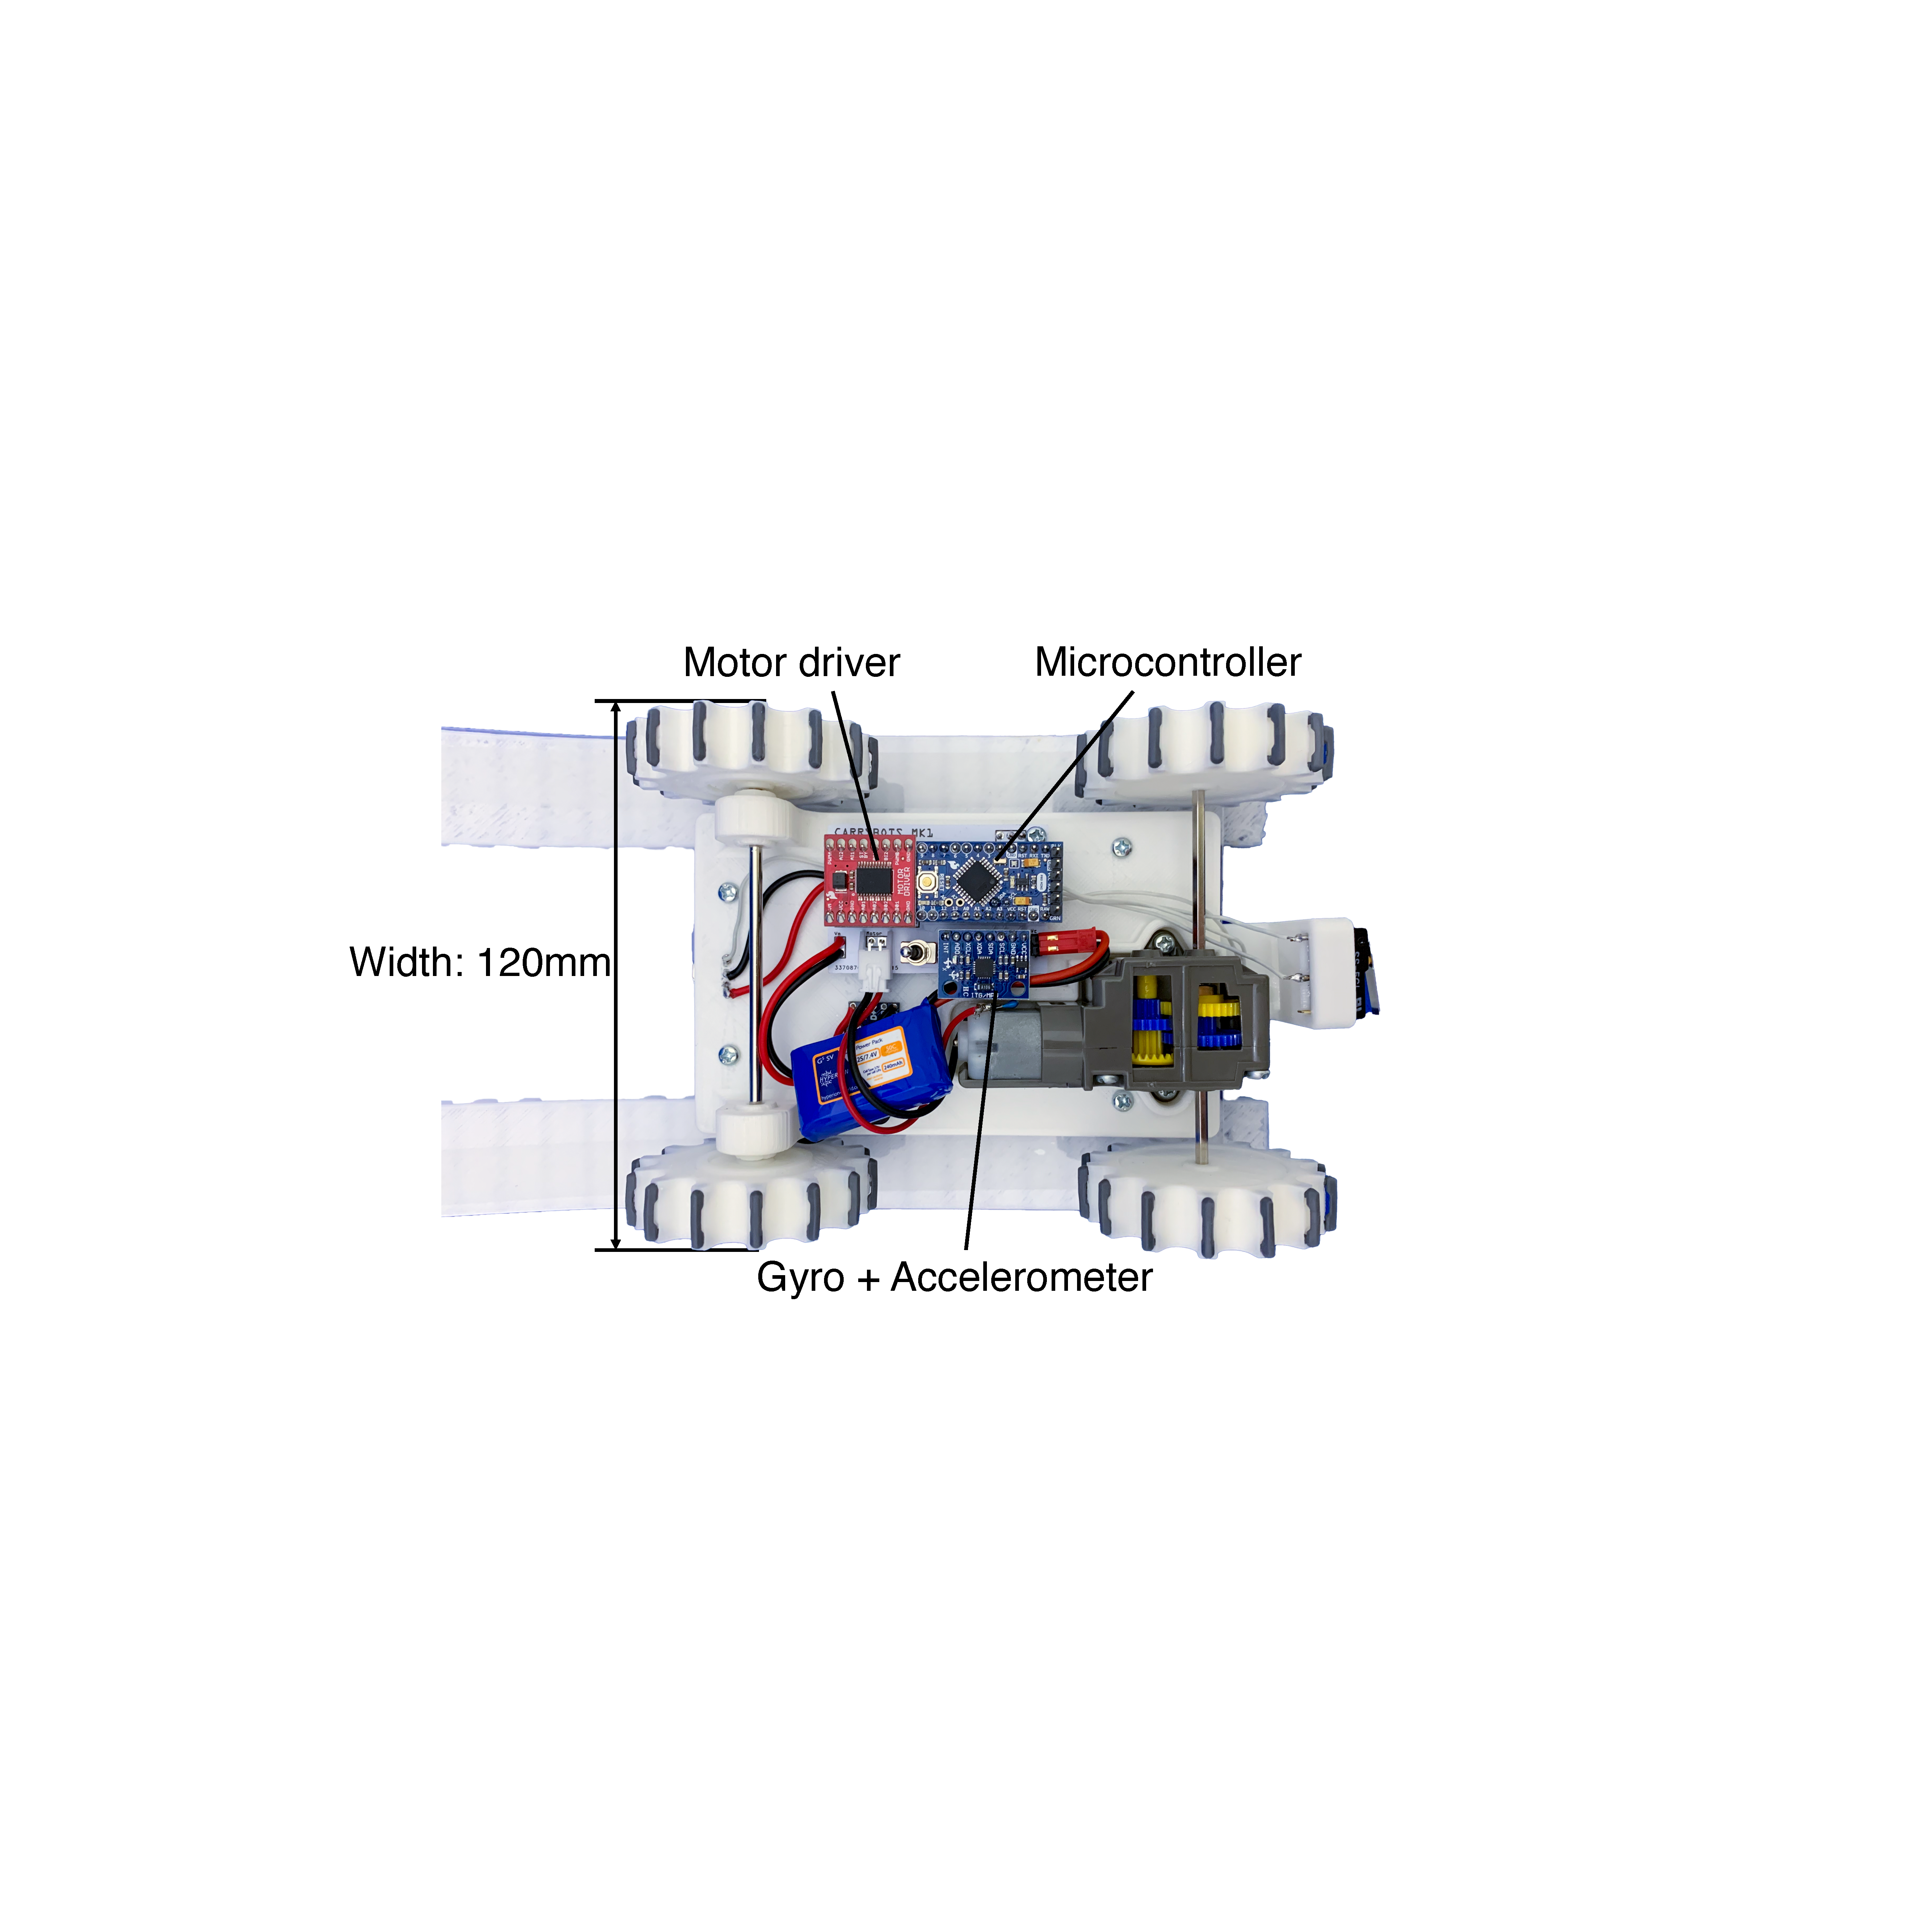
\includegraphics[width=0.9\columnwidth]{figures/carrybot-bottom.pdf}
  \subcaption{Bottom view}
  \label{fig:bottom}
 \end{minipage}
 \caption{Mechanical structure of the robot}
 \label{fig:carrybot}
\end{figure}
